% !TEX root = ../Dokumentation.tex
\subsection{Objekterkennung}

\subsubsection{Containererkennung}
Die Containererkennung hat das Ziel die richtigen Container zu erkennen und das genaue positionieren des Fahrzeuges zu ermöglichen. Dabei wird die Containererkennung wieder in zwei Teilaufgaben aufgeteilt. Die Containererkennung grob ist für die Erkennung der richtigen Farbe (und Form) zuständig. Die Containererkennung präzise ist für das Positionieren des Fahrzeuges notwendig. Diese zwei Fälle werden separat angeschaut.\\
\\
\textbf{Containererkennung präzise}\\
\\
\textbf{Funktionsbeschrieb}\\
Die präzise Containererkennung wird für das genaue Stoppen des Fahrzeuges gebraucht. Dieses Modul gibt den Trigger zum anhalten.\\
\\
\textbf{Komponentenbeschrieb}\\
Die Container Erkennung wird mit Hilfe von Distanzsensoren realisiert. Dafür sind Infrarot Distanzmesser oder Infrarot Reflexkoppler vorgesehen. Diese werden auf der rechten Seite des Fahrzeuges befestigt. Sobald ein Objekt in der Nähe ist ändert sich der Spannungswert, was einer Distanzänderung gleichkommt. 
\begin{figure} [hbp]
	\centering
	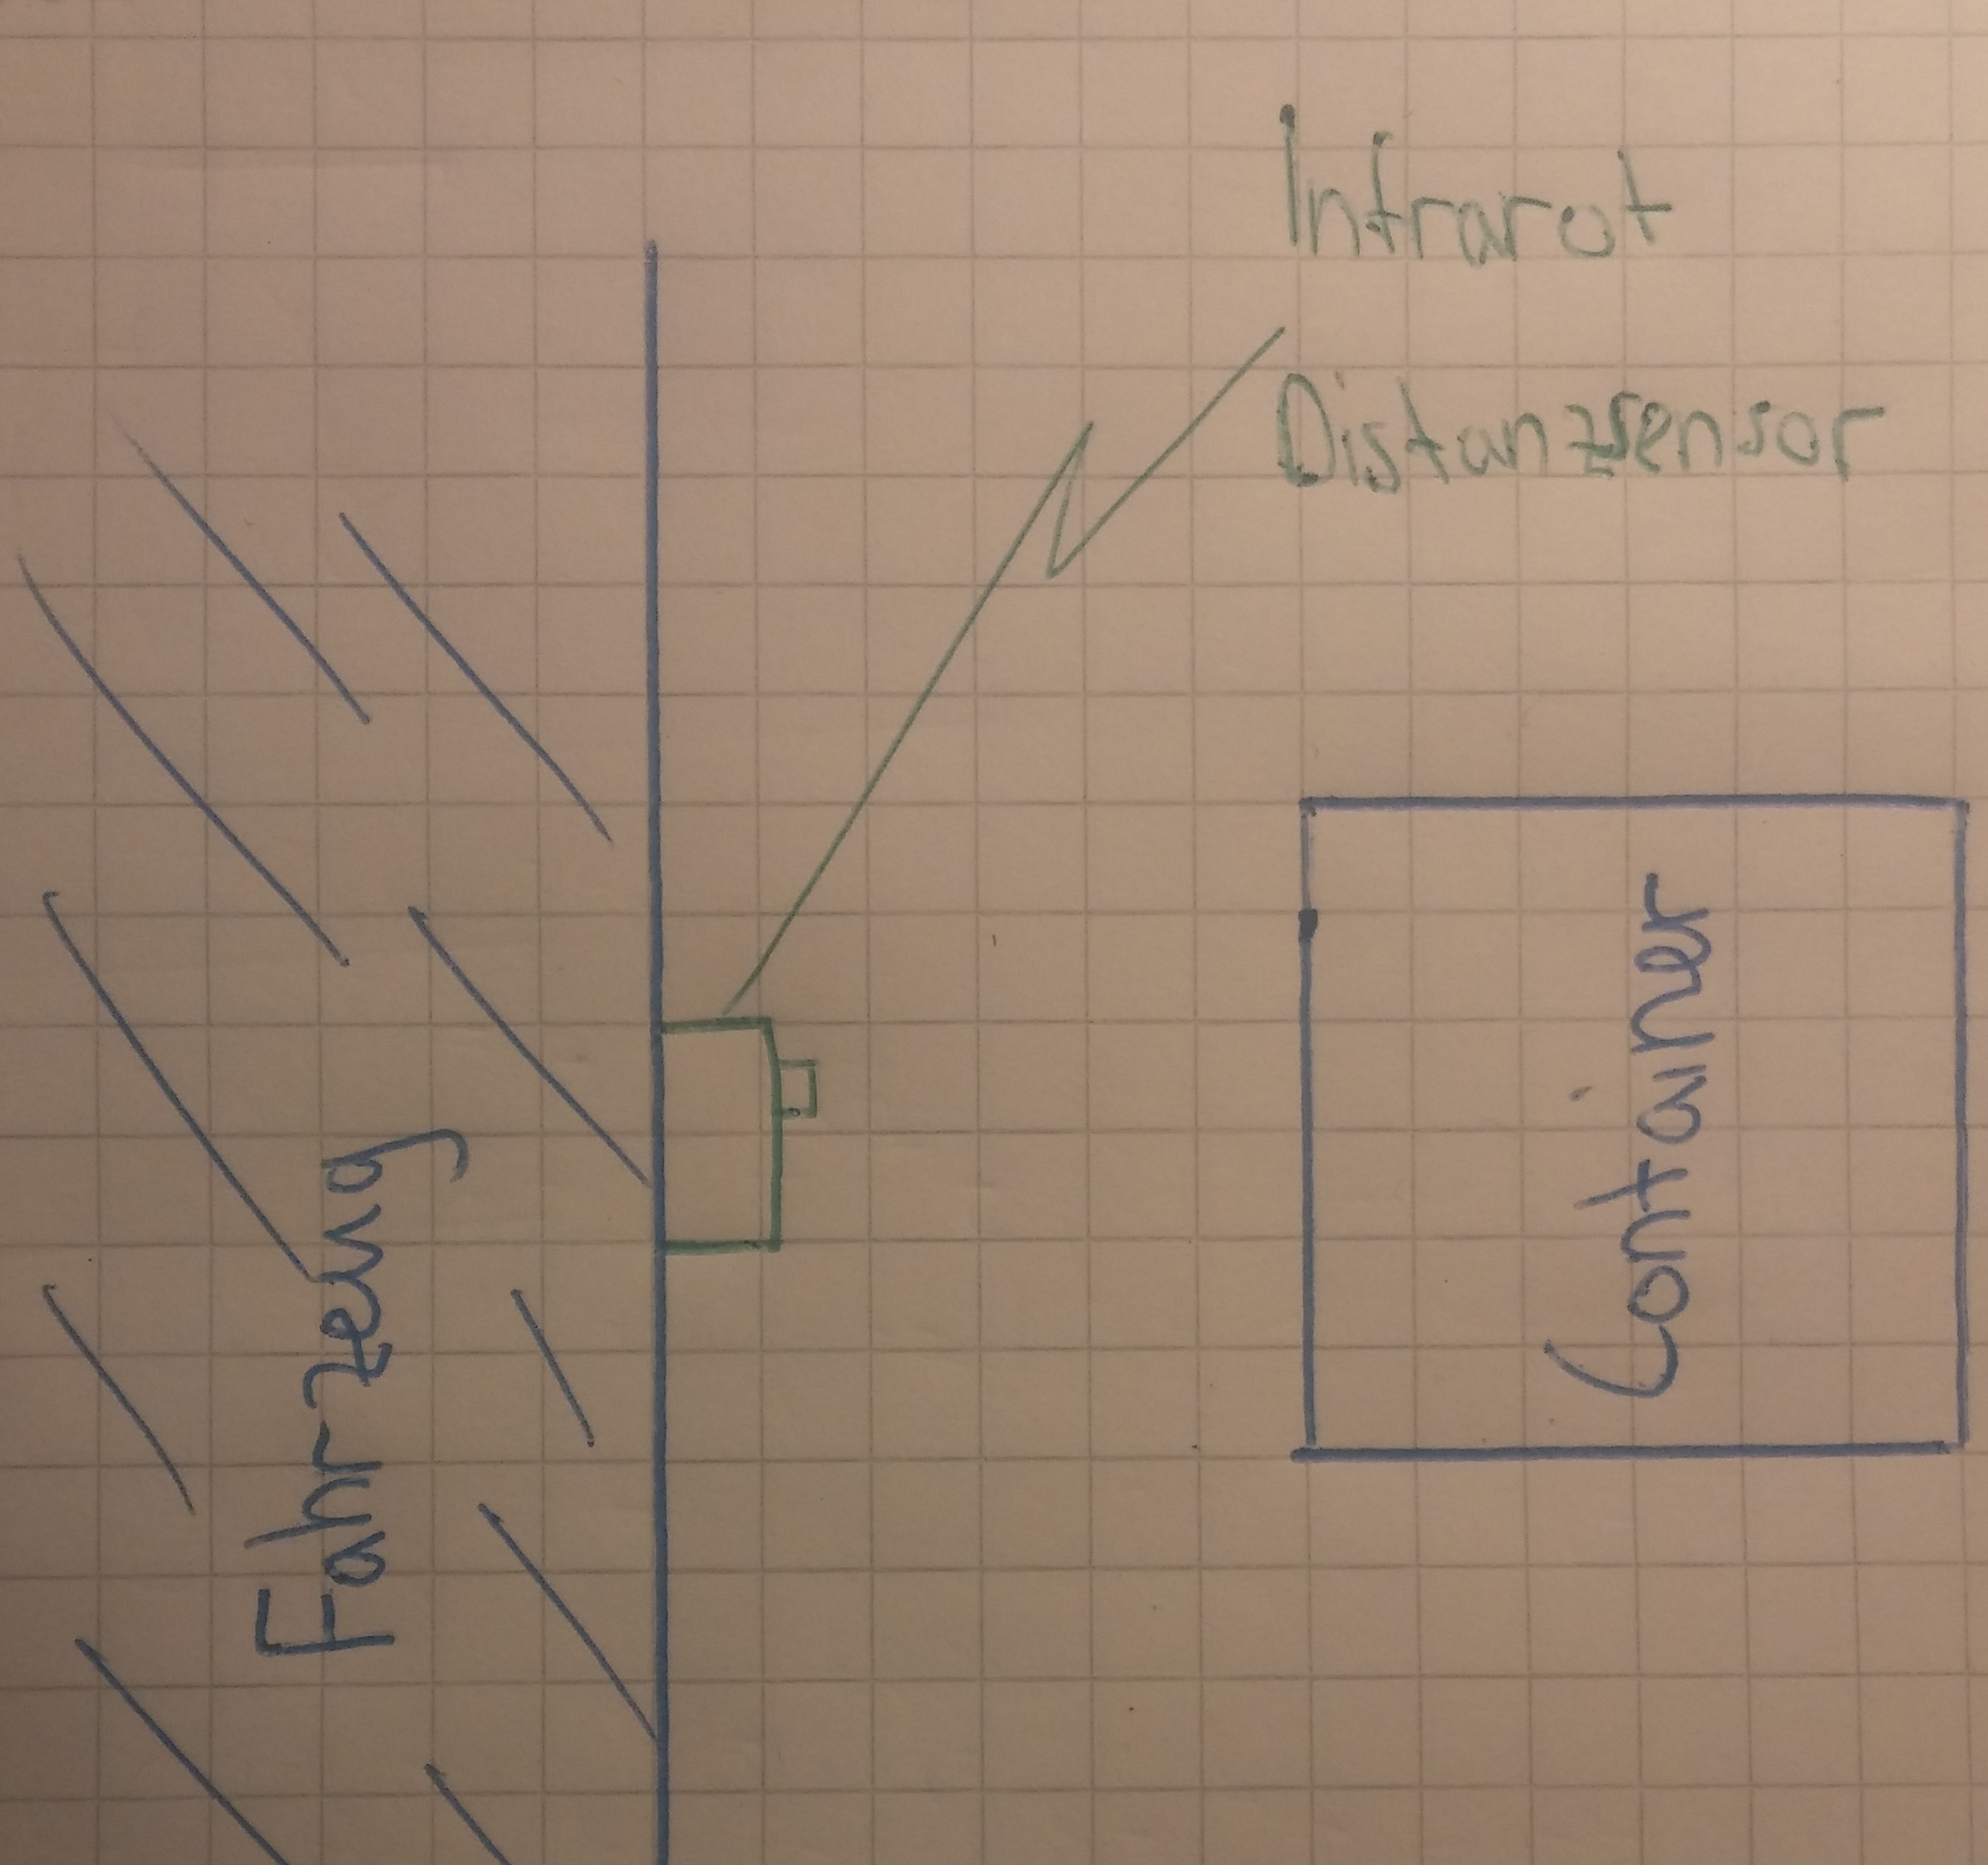
\includegraphics[width=0.35\textwidth]{./Images/InfrarotContainererkennung.png}
	\caption{Beispielhafte Containererkennung mit einem Infrarotsensor}
\end{figure}\\
\\
\textbf{Begründung}
\\
Die Positionierung mit einem Infrarotsensor ist die Ideale Lösung. Sie ist einfach zu realisieren im Vergleich zu einer Kamera oder einem Farbesensor und präziserer als ein Ultraschallsensor.\\
\\
\textbf{Testergebnisse}\\
Für die Ermittlung des besten Sensors wurde ein Ultraschall und Infrarotsensor als Funktionsmuster getestet. Der relativ grosse "Empfangswinkel", welcher der Ultraschallsensor aufweist, ist in dieser Anwendung nicht gewollt. Der Infrarotsensor ist diesbezüglich besser. Dieser ist jedoch Lichtempfindlich, jedoch sollte dieses Problem gelöst werden können.\
\\
\subsubsection{Rechtsvortritt}
\textbf{Funktionsbeschrieb}

\textbf{Komponentenbeschrieb}
\textbf{Begründung}
Wenn benötigt
\textbf{Berechnungen}
\textbf{Testergebnisse}